% Created by tikzDevice version 0.12.6 on 2026-08-10 06:15:20
% !TEX encoding = UTF-8 Unicode
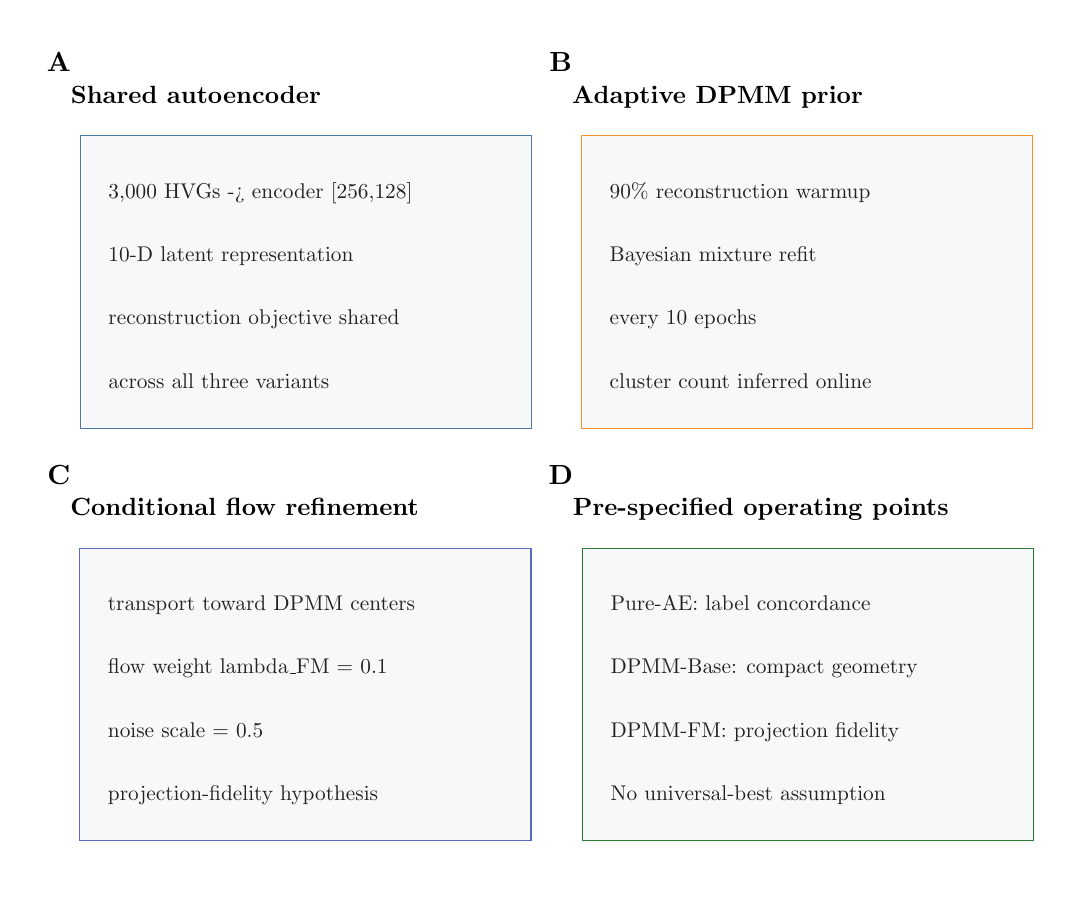
\begin{tikzpicture}[x=1pt,y=1pt]
\definecolor{fillColor}{RGB}{255,255,255}
\path[use as bounding box,fill=fillColor,fill opacity=0.00] (0,0) rectangle (373.73,309.06);
\begin{scope}
\path[clip] (  0.00,  0.00) rectangle (373.73,309.06);
\definecolor{drawColor}{RGB}{255,255,255}
\definecolor{fillColor}{RGB}{255,255,255}

\path[draw=drawColor,line width= 0.6pt,line join=round,line cap=round,fill=fillColor] (  0.00,  0.00) rectangle (373.73,309.06);
\end{scope}
\begin{scope}
\path[clip] (  5.50,154.53) rectangle (186.86,303.56);
\definecolor{drawColor}{RGB}{255,255,255}
\definecolor{fillColor}{RGB}{255,255,255}

\path[draw=drawColor,line width= 0.6pt,line join=round,line cap=round,fill=fillColor] (  5.50,154.53) rectangle (186.86,303.56);
\end{scope}
\begin{scope}
\path[clip] (186.86,154.53) rectangle (368.23,303.56);
\definecolor{drawColor}{RGB}{255,255,255}
\definecolor{fillColor}{RGB}{255,255,255}

\path[draw=drawColor,line width= 0.6pt,line join=round,line cap=round,fill=fillColor] (186.86,154.53) rectangle (368.23,303.56);
\end{scope}
\begin{scope}
\path[clip] (  4.92,154.96) rectangle (187.44,303.13);

\path[] (  4.92,154.96) rectangle (187.44,303.13);
\end{scope}
\begin{scope}
\path[clip] ( 15.61,156.96) rectangle (185.44,279.82);
\definecolor{drawColor}{RGB}{78,121,167}
\definecolor{fillColor}{RGB}{247,248,250}

\path[draw=drawColor,line width= 0.5pt,fill=fillColor] ( 19.01,164.33) rectangle (182.05,269.99);
\definecolor{drawColor}{RGB}{34,34,34}

\node[text=drawColor,anchor=base west,inner sep=0pt, outer sep=0pt, scale=  0.77] at ( 29.20,247.50) {3,000 HVGs -> encoder [256,128]};

\node[text=drawColor,anchor=base west,inner sep=0pt, outer sep=0pt, scale=  0.77] at ( 29.20,224.57) {10-D latent representation};

\node[text=drawColor,anchor=base west,inner sep=0pt, outer sep=0pt, scale=  0.77] at ( 29.20,201.63) {reconstruction objective shared};

\node[text=drawColor,anchor=base west,inner sep=0pt, outer sep=0pt, scale=  0.77] at ( 29.20,178.70) {across all three variants};
\end{scope}
\begin{scope}
\path[clip] (  0.00,  0.00) rectangle (373.73,309.06);
\definecolor{drawColor}{RGB}{0,0,0}

\node[text=drawColor,anchor=base west,inner sep=0pt, outer sep=0pt, scale=  0.90] at ( 15.61,281.81) {\bfseries Shared autoencoder};
\end{scope}
\begin{scope}
\path[clip] (  0.00,  0.00) rectangle (373.73,309.06);
\definecolor{drawColor}{RGB}{0,0,0}

\node[text=drawColor,anchor=base,inner sep=0pt, outer sep=0pt, scale=  1.00] at ( 11.26,293.12) {\bfseries A};
\end{scope}
\begin{scope}
\path[clip] (186.54,154.96) rectangle (368.55,303.13);

\path[] (186.54,154.96) rectangle (368.55,303.13);
\end{scope}
\begin{scope}
\path[clip] (196.72,156.96) rectangle (366.55,279.82);
\definecolor{drawColor}{RGB}{242,142,43}
\definecolor{fillColor}{RGB}{247,248,250}

\path[draw=drawColor,line width= 0.5pt,fill=fillColor] (200.11,164.33) rectangle (363.15,269.99);
\definecolor{drawColor}{RGB}{34,34,34}

\node[text=drawColor,anchor=base west,inner sep=0pt, outer sep=0pt, scale=  0.77] at (210.30,247.50) {90{\%} reconstruction warmup};

\node[text=drawColor,anchor=base west,inner sep=0pt, outer sep=0pt, scale=  0.77] at (210.30,224.57) {Bayesian mixture refit};

\node[text=drawColor,anchor=base west,inner sep=0pt, outer sep=0pt, scale=  0.77] at (210.30,201.63) {every 10 epochs};

\node[text=drawColor,anchor=base west,inner sep=0pt, outer sep=0pt, scale=  0.77] at (210.30,178.70) {cluster count inferred online};
\end{scope}
\begin{scope}
\path[clip] (  0.00,  0.00) rectangle (373.73,309.06);
\definecolor{drawColor}{RGB}{0,0,0}

\node[text=drawColor,anchor=base west,inner sep=0pt, outer sep=0pt, scale=  0.90] at (196.72,281.81) {\bfseries Adaptive DPMM prior};
\end{scope}
\begin{scope}
\path[clip] (  0.00,  0.00) rectangle (373.73,309.06);
\definecolor{drawColor}{RGB}{0,0,0}

\node[text=drawColor,anchor=base,inner sep=0pt, outer sep=0pt, scale=  1.00] at (192.63,293.12) {\bfseries B};
\end{scope}
\begin{scope}
\path[clip] (  5.50,  5.50) rectangle (186.86,154.53);
\definecolor{drawColor}{RGB}{255,255,255}
\definecolor{fillColor}{RGB}{255,255,255}

\path[draw=drawColor,line width= 0.6pt,line join=round,line cap=round,fill=fillColor] (  5.50,  5.50) rectangle (186.86,154.53);
\end{scope}
\begin{scope}
\path[clip] (186.86,  5.50) rectangle (368.23,154.53);
\definecolor{drawColor}{RGB}{255,255,255}
\definecolor{fillColor}{RGB}{255,255,255}

\path[draw=drawColor,line width= 0.6pt,line join=round,line cap=round,fill=fillColor] (186.86,  5.50) rectangle (368.23,154.53);
\end{scope}
\begin{scope}
\path[clip] (  5.11,  5.93) rectangle (187.25,154.10);

\path[] (  5.11,  5.93) rectangle (187.25,154.10);
\end{scope}
\begin{scope}
\path[clip] ( 15.42,  7.93) rectangle (185.25,130.79);
\definecolor{drawColor}{RGB}{92,107,192}
\definecolor{fillColor}{RGB}{247,248,250}

\path[draw=drawColor,line width= 0.5pt,fill=fillColor] ( 18.81, 15.30) rectangle (181.85,120.96);
\definecolor{drawColor}{RGB}{34,34,34}

\node[text=drawColor,anchor=base west,inner sep=0pt, outer sep=0pt, scale=  0.77] at ( 29.00, 98.47) {transport toward DPMM centers};

\node[text=drawColor,anchor=base west,inner sep=0pt, outer sep=0pt, scale=  0.77] at ( 29.00, 75.54) {flow weight lambda{\_{}}FM = 0.1};

\node[text=drawColor,anchor=base west,inner sep=0pt, outer sep=0pt, scale=  0.77] at ( 29.00, 52.60) {noise scale = 0.5};

\node[text=drawColor,anchor=base west,inner sep=0pt, outer sep=0pt, scale=  0.77] at ( 29.00, 29.67) {projection-fidelity hypothesis};
\end{scope}
\begin{scope}
\path[clip] (  0.00,  0.00) rectangle (373.73,309.06);
\definecolor{drawColor}{RGB}{0,0,0}

\node[text=drawColor,anchor=base west,inner sep=0pt, outer sep=0pt, scale=  0.90] at ( 15.42,132.78) {\bfseries Conditional flow refinement};
\end{scope}
\begin{scope}
\path[clip] (  0.00,  0.00) rectangle (373.73,309.06);
\definecolor{drawColor}{RGB}{0,0,0}

\node[text=drawColor,anchor=base,inner sep=0pt, outer sep=0pt, scale=  1.00] at ( 11.26,144.09) {\bfseries C};
\end{scope}
\begin{scope}
\path[clip] (186.22,  5.93) rectangle (368.87,154.10);

\path[] (186.22,  5.93) rectangle (368.87,154.10);
\end{scope}
\begin{scope}
\path[clip] (197.04,  7.93) rectangle (366.87,130.79);
\definecolor{drawColor}{RGB}{46,125,50}
\definecolor{fillColor}{RGB}{247,248,250}

\path[draw=drawColor,line width= 0.5pt,fill=fillColor] (200.43, 15.30) rectangle (363.47,120.96);
\definecolor{drawColor}{RGB}{34,34,34}

\node[text=drawColor,anchor=base west,inner sep=0pt, outer sep=0pt, scale=  0.77] at (210.62, 98.47) {Pure-AE: label concordance};

\node[text=drawColor,anchor=base west,inner sep=0pt, outer sep=0pt, scale=  0.77] at (210.62, 75.54) {DPMM-Base: compact geometry};

\node[text=drawColor,anchor=base west,inner sep=0pt, outer sep=0pt, scale=  0.77] at (210.62, 52.60) {DPMM-FM: projection fidelity};

\node[text=drawColor,anchor=base west,inner sep=0pt, outer sep=0pt, scale=  0.77] at (210.62, 29.67) {No universal-best assumption};
\end{scope}
\begin{scope}
\path[clip] (  0.00,  0.00) rectangle (373.73,309.06);
\definecolor{drawColor}{RGB}{0,0,0}

\node[text=drawColor,anchor=base west,inner sep=0pt, outer sep=0pt, scale=  0.90] at (197.04,132.78) {\bfseries Pre-specified operating points};
\end{scope}
\begin{scope}
\path[clip] (  0.00,  0.00) rectangle (373.73,309.06);
\definecolor{drawColor}{RGB}{0,0,0}

\node[text=drawColor,anchor=base,inner sep=0pt, outer sep=0pt, scale=  1.00] at (192.63,144.09) {\bfseries D};
\end{scope}
\end{tikzpicture}
